\documentclass[11pt]{amsart}

\usepackage{amsmath,amsthm}
\usepackage{amssymb}
\usepackage{graphicx}
\usepackage{enumerate}
\usepackage{fullpage}
% \usepackage{euscript}
% \makeatletter
\usepackage{pdfpages}

% \nopagenumbers
\usepackage{verbatim}
\usepackage{color}
\usepackage{hyperref}

\usepackage{fullpage,tikz,float}
%\usepackage{times} %, mathtime}

\textheight=600pt %574pt
\textwidth=480pt %432pt
\oddsidemargin=15pt %18.88pt
\evensidemargin=18.88pt
\topmargin=10pt %14.21pt

\parskip=1pt %2pt

% define theorem environments
\newtheorem{theorem}{Theorem}    %[section]
%\def\thetheorem{\unskip}
\newtheorem{proposition}[theorem]{Proposition}
%\def\theproposition{\unskip}
\newtheorem{conjecture}[theorem]{Conjecture}
\def\theconjecture{\unskip}
\newtheorem{corollary}[theorem]{Corollary}
\newtheorem{lemma}[theorem]{Lemma}
\newtheorem{sublemma}[theorem]{Sublemma}
\newtheorem{fact}[theorem]{Fact}
\newtheorem{observation}[theorem]{Observation}
%\def\thelemma{\unskip}
\theoremstyle{definition}
\newtheorem{definition}{Definition}
%\def\thedefinition{\unskip}
\newtheorem{notation}[definition]{Notation}
\newtheorem{remark}[definition]{Remark}
% \def\theremark{\unskip}
\newtheorem{question}[definition]{Question}
\newtheorem{questions}[definition]{Questions}
%\def\thequestion{\unskip}
\newtheorem{example}[definition]{Example}
%\def\theexample{\unskip}
\newtheorem{problem}[definition]{Problem}
\newtheorem{exercise}[definition]{Exercise}

\numberwithin{theorem}{section}
\numberwithin{definition}{section}
\numberwithin{equation}{section}

\def\reals{{\mathbb R}}
\def\torus{{\mathbb T}}
\def\integers{{\mathbb Z}}
\def\rationals{{\mathbb Q}}
\def\naturals{{\mathbb N}}
\def\complex{{\mathbb C}\/}
\def\distance{\operatorname{distance}\,}
\def\support{\operatorname{support}\,}
\def\dist{\operatorname{dist}\,}
\def\Span{\operatorname{span}\,}
\def\degree{\operatorname{degree}\,}
\def\kernel{\operatorname{kernel}\,}
\def\dim{\operatorname{dim}\,}
\def\codim{\operatorname{codim}}
\def\trace{\operatorname{trace\,}}
\def\dimension{\operatorname{dimension}\,}
\def\codimension{\operatorname{codimension}\,}
\def\nullspace{\scriptk}
\def\kernel{\operatorname{Ker}}
\def\p{\partial}
\def\Re{\operatorname{Re\,} }
\def\Im{\operatorname{Im\,} }
\def\ov{\overline}
\def\eps{\varepsilon}
\def\lt{L^2}
\def\curl{\operatorname{curl}}
\def\divergence{\operatorname{div}}
\newcommand{\norm}[1]{ \|  #1 \|}
\def\expect{\mathbb E}
\def\bull{$\bullet$\ }
\def\det{\operatorname{det}}
\def\Det{\operatorname{Det}}
\def\rank{\mathbf r}
\def\diameter{\operatorname{diameter}}

\def\t2{\tfrac12}

\newcommand{\abr}[1]{ \langle  #1 \rangle}

\def\newbull{\medskip\noindent $\bullet$\ }
\def\field{{\mathbb F}}
\def\cc{C_c}



% \renewcommand\forall{\ \forall\,}

% \newcommand{\Norm}[1]{ \left\|  #1 \right\| }
\newcommand{\Norm}[1]{ \Big\|  #1 \Big\| }
\newcommand{\set}[1]{ \left\{ #1 \right\} }
%\newcommand{\ifof}{\Leftrightarrow}
\def\one{{\mathbf 1}}
\newcommand{\modulo}[2]{[#1]_{#2}}

\def\bd{\operatorname{bd}\,}
\def\cl{\text{cl}}
\def\nobull{\noindent$\bullet$\ }

\def\scriptf{{\mathcal F}}
\def\scriptq{{\mathcal Q}}
\def\scriptg{{\mathcal G}}
\def\scriptm{{\mathcal M}}
\def\scriptb{{\mathcal B}}
\def\scriptc{{\mathcal C}}
\def\scriptt{{\mathcal T}}
\def\scripti{{\mathcal I}}
\def\scripte{{\mathcal E}}
\def\scriptv{{\mathcal V}}
\def\scriptw{{\mathcal W}}
\def\scriptu{{\mathcal U}}
\def\scriptS{{\mathcal S}}
\def\scripta{{\mathcal A}}
\def\scriptr{{\mathcal R}}
\def\scripto{{\mathcal O}}
\def\scripth{{\mathcal H}}
\def\scriptd{{\mathcal D}}
\def\scriptl{{\mathcal L}}
\def\scriptn{{\mathcal N}}
\def\scriptp{{\mathcal P}}
\def\scriptk{{\mathcal K}}
\def\scriptP{{\mathcal P}}
\def\scriptj{{\mathcal J}}
\def\scriptz{{\mathcal Z}}
\def\scripts{{\mathcal S}}
\def\scriptx{{\mathcal X}}
\def\scripty{{\mathcal Y}}
\def\frakv{{\mathfrak V}}
\def\frakG{{\mathfrak G}}
\def\aff{\operatorname{Aff}}
\def\frakB{{\mathfrak B}}
\def\frakC{{\mathfrak C}}

\def\symdif{\,\Delta\,}
\def\mustar{\mu^*}
\def\muplus{\mu^+}

\def\soln{\noindent {\bf Solution.}\ }


%\pagestyle{empty}
%\setlength{\parindent}{0pt}

\begin{document}

\begin{center}{\bf Math 215A --- UCB, Spring 2017 --- William Guss} \\
Partners: Alekos, Chris \\
Selected Problems: 2
\end{center}


\medskip \noindent {\bf (3.1)} \emph{Show that the following sets form smooth submanifolds of the real vector space of $n \times n$ matrices with real coefficents:}
\begin{equation*}
	GL(n), SL(n), O(n), SO(n) \subset Mat(n,n).
\end{equation*}
\emph{Determine\footnote{Not sure if you also want us to prove this.} their dimensions, the number of components and show that multiplication and inversion are smooth maps for these groups.}\\

\noindent \emph{Solution.} Before we consider the subsets given, we verify an assumption of the problem.

\begin{lemma}
$Mat(n,n)$ is a smooth manifold.
\end{lemma}
\begin{proof}
We will first that this space is a smooth manifold. To do so, consider that $Mat(n,n) = \mathbb{R}^n \otimes \mathbb{R}^n$ and we can give the diffeomorphism:
	\begin{equation*}
		Mat(n,n) \ni M \mapsto (M_{floor(i/n),(i \mod n)})_{i=1}^{n^2} \in \mathbb{R}^{n^2}
	\end{equation*}
	by rearrangement of coordinates. Since $\mathbb{R}^{n^2}$ is a smooth manifold, we have that $Mat(n,n)$ is a smooth manifold of dimension $n^2.$ 
\end{proof}

\begin{lemma}
	If $M$ is a smooth manifold and $N \subset M$ is an open subset then $N$ is a smooth submanifold of $M$ and $dim(M) = dim(N).$
\end{lemma}
\begin{proof}
 First if $N \subset M$ then in the inherited subspace topology $N$ is also Hausdorff and second countable from standard topology. Consider the following collection of charts
 \begin{equation*}
  	\scripta_N = \{U\cap N, \phi|_{U\cap N}\mathrel{}\Big|\mathrel{} U \cap N \neq \emptyset (U, \phi) \in \scripta_M \}.
  \end{equation*} 
  Since $U \cap N$ is open $\phi|_{U\cap N}$ is a diffeomorphism to $\mathbb{R}^{\dim(M)}$. Furthermore $N$ is covered as the atlas $\scripta_M$ covers $M$ with the union of its domain collection. Therefore $\scripta_N$ forms a smooth atlas on $N$.  Thereafter yield the smooth structure under the equivalence class of compatible atlases, and then $N$ is a smooth manifold with dimension $\dim(M).$
\end{proof}
 

\noindent We will now address each group by case.
\begin{itemize}
	\item $GL(n).$ Recall that the general linear group is defined such that 
	\begin{equation*}
		GL(n) = \{ M \in Mat(n,n)\mathrel{}\Big|\mathrel{} det(M) \neq 0\},
	\end{equation*} We claim that this space is a submanifold. To see this, take the map $\det: M \to \mathbb{R}$ and under the standard topology of $Mat(n,n)$, $\det$ is continuous map. This is true as $\det$ is the composition of multiplication and addition operations on components of elements of $M$. Since $GL(n) = \det^{-1}[(-\infty, 0) \cup (0, \infty)]$ we have that $GL(n)$ is open by definition of continuity. Therefore $GL(n)$ is a smooth submanifold of $Mat(n,n)$ inheriting the subspace topology and intersecting smooth structure of $Mat(n,n)$ by the previous lemma. \\

	\noindent We will now show that $GL(n)$ is a Lie group. First consider matrix multiplication as an operation in $GL(n)$, we will recall from linear algebra that this operation is closed and $GL(n)$ forms a group. As the product of smooth manifolds is smooth, it suffices to show that $mul: GL(n) \times GL(n) \to GL(n)$ is a smooth map. Take $(U, \phi)$ from the smooth structure on $GL(n) \times GL(n)$ so that $\phi: GL(n) \times GL(n) \to \mathbb{R}^{n^2} \times \mathbb{R}^{n^2}$. Then without loss of generality there is a $V = mul(U)$ and $\psi$ so that $(V, \psi)$ is in the smooth structure of th codomain $GL(n) = mul(GL(n), GL(n)).$ We will consider the composition of these maps in local coordinates; that is
	\begin{equation*}
		\psi \circ mul \circ \phi^{-1}: (x^1, x^2) \mapsto \psi \circ \left(\sum_{k=1}^m \phi_1^{-1}(x^1_{ik})\cdot \phi_2^{-1}(x^2_{kj})\right)_{i,j}
	\end{equation*}
	is the composition of smooth operations. In particular multiplication and summation in $\mathbb{R}^{n^2}$ are smooth and continuous. Therefore $mul$ is smooth. 

	Now consider the group inverse $inv: GL(n) \to GL(n)$ and again take an arbitrary $(U, \phi)$ but this time in $GL(n)$. Then let $V = inv(V)$ so that $(V, \psi)$ is without loss of generality a chart in the smooth structure of $GL(n).$ We will consider the the composition of these maps in local coordinates; that is,
	\begin{equation*}
		\psi \circ inv \circ \phi^{-1}: x \mapsto \psi \circ \left(\frac{det((\phi^{-1}(x)_{[ij]})}{det(\phi_1^{-1}(x))} \right)_{i,j}
	\end{equation*}
	is the composition of smooth operations. In particular the determinant of matrices $\phi^{-1}(x)_{[ij]})$\footnote{Removing the $i$th row and $j$th column.} is a polynomial function of the elements and so it is a smooth function. Therefore the map is smooth. This makes $GL(n)$ a Lie group.

	$GL(n)$ has two connected components.

	\item $O(n)$. To show that the orthogonal group is a manifold we will use theorems presented in class. In particular, consider the smooth map 
	$\phi(M) = M^TM - id$ to $Mat(n,n)$. Then clearly $\phi^{-1}(0) = O(n)$ so using that the inverse of a regular value is a submanifold (smooth) we get that $O(n)$ is a manifold. Since $O(n)$ is an embedded submanifold of $GL(n)$ so we yield that the group operations on $O(n)$ are aslo smooth and $O(n)$ is a Lie group. The key is here is that $mul(O(n), O(n)) \subset O(n)$ and $inv(O(n)) \subset O(n).$

	$O(n)$ has two connected components which are necissary in the classification of $GL(n).$ 

	As for the dimension of $O(n),$ we need consider the kernal dimension of the linear map $D \phi$ of tangent spaces in concordance with the lectures.   In this case the matrix derivative of $\phi$ is
	$D (M^T M) = M^T \cdot + (M^T \cdot)^T$ and thus the operator on tangent spaces is a symmetric operator by the invertibility of $M$.  Therefore the dimnension of $O(n)$ is that of the set of difference between $dim(GL(n))$ and that of $n\times n$ symmetric matrices. We consider combinations of free elements in matrices and yield
	\begin{equation*}
		dim(O(n)) =n^2 -\sum_{k=1}^n k = n(n+1)/2.
	\end{equation*}

	\item $SL(n).$ Consider the special linear group. We will show that is a closed subanifold of $GL(n)$ by showing that $1$ is a regular value of $det: Mat(n,n) \to \mathbb{R}.$ First by definitio we have $SL(n) = f^{-1}(1).$ To show that $1$ is a regular value of $det$, suppose there is some matrix $A \in SL(n)$ which is a critical point. Then every matrix $A_{[ij]}$ where we adopt notation from earlier must have determinant $0$. But the only possible such matrix herefore has determinant $0$, and so all points of $SL(n)$ are not critical and since $SL(N) = f^{-1}(1),$ the special linear group is a closed submanifold of $GL(n).$  

	Furthermore, $SL(n)$ inherits the the smoothness of matrix multiplication and inversion from $GL(n)$

	As for connected components, if $det(A) > 0, A \in GL(n)$ then $A$ path connected to $O^{+}(n).$ Since path components and components coincide on smooth manifolds, the connectedness of $O^{+}(n)$ yields $SL(n)$ conncted. This space has dimension $n^2 -1.$

	\item $SO(n)$. Since $SO(n)$ is a connected subset of $O(n)$, and the inverse image of $\{1\} \subset \{\pm 1\}$ through $det$ we have that it is a submanifold of $O(n).$ Again $SO(n)$ inherits the smoothness of the group operations from $GL(n).$
\end{itemize}

\medskip \noindent {\bf (3.2)}  \emph{Show that the Mobiusband M} admits a non-vanishing vecotr field but is not parallelizable. 

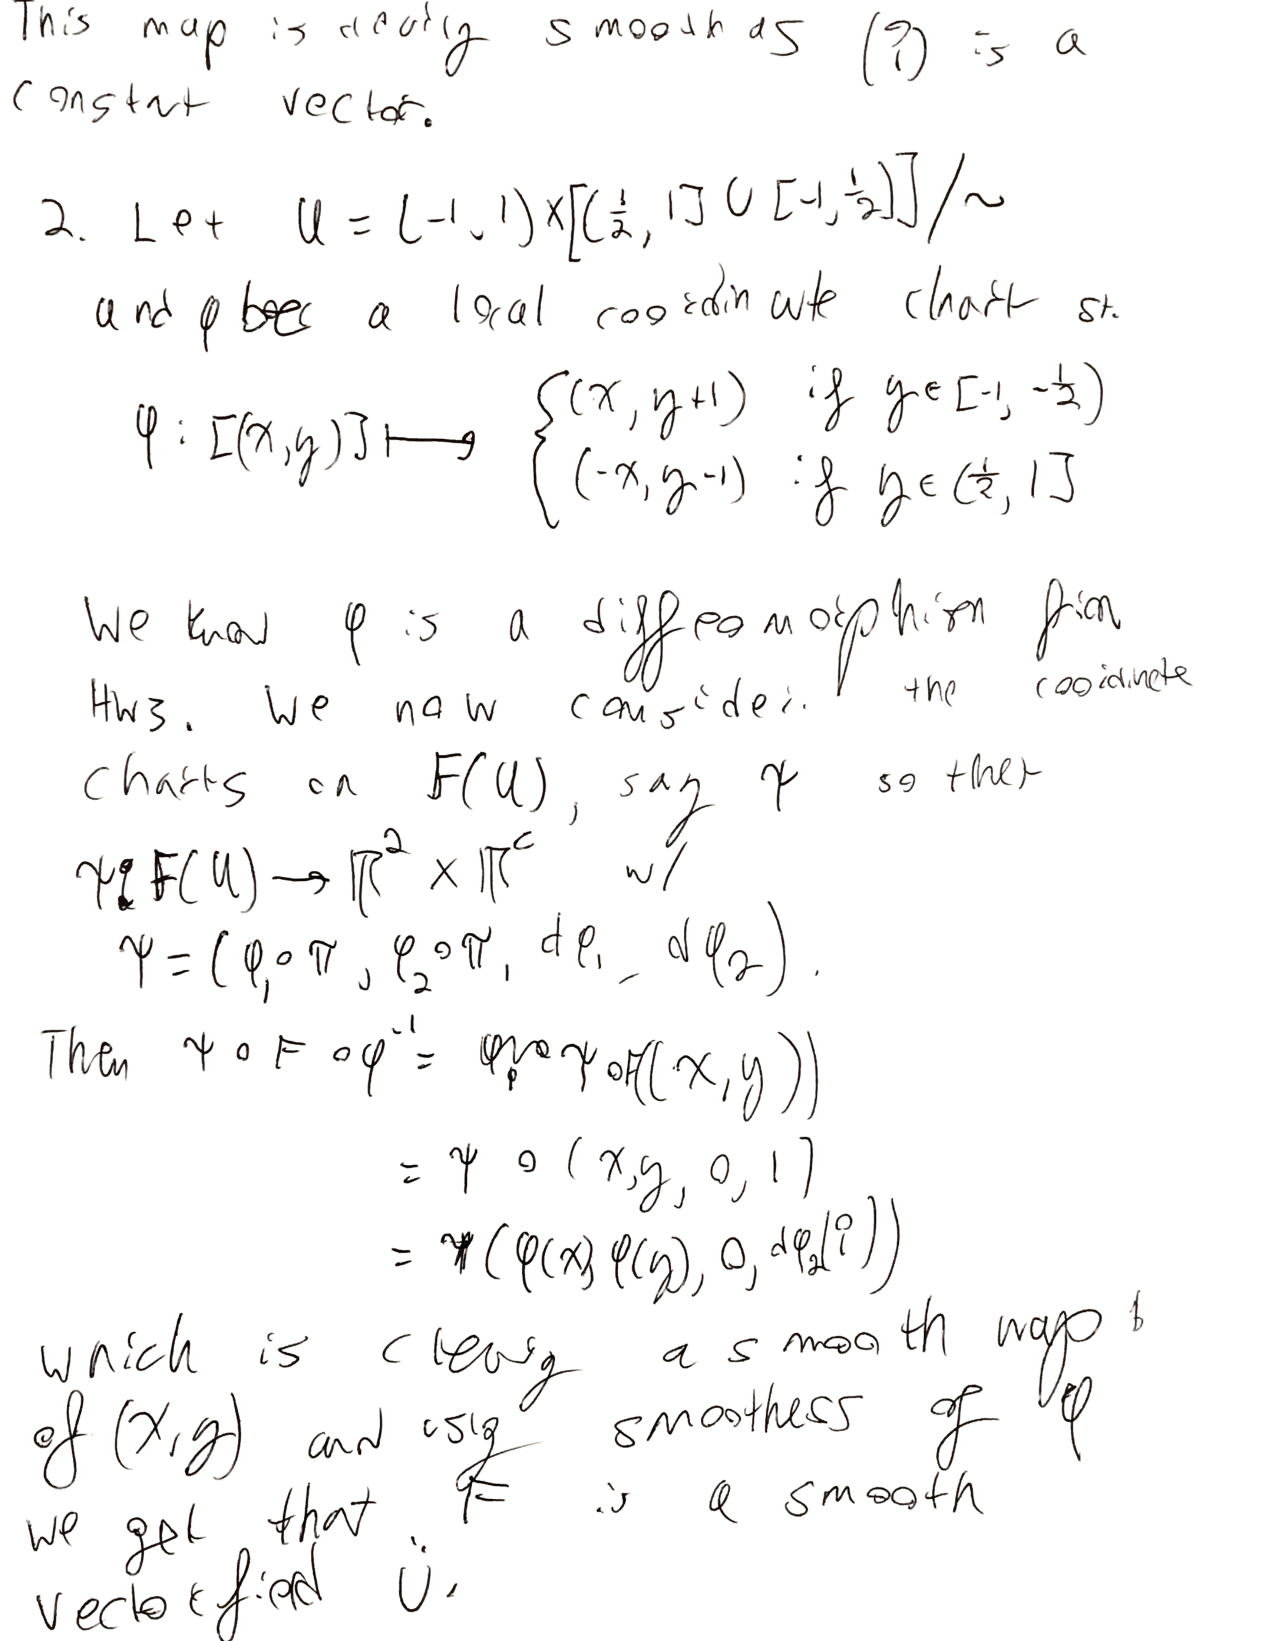
\includepdf[pages={1}]{yes.pdf}	

\includepdf[pages={2}]{yes.pdf}	
\newpage
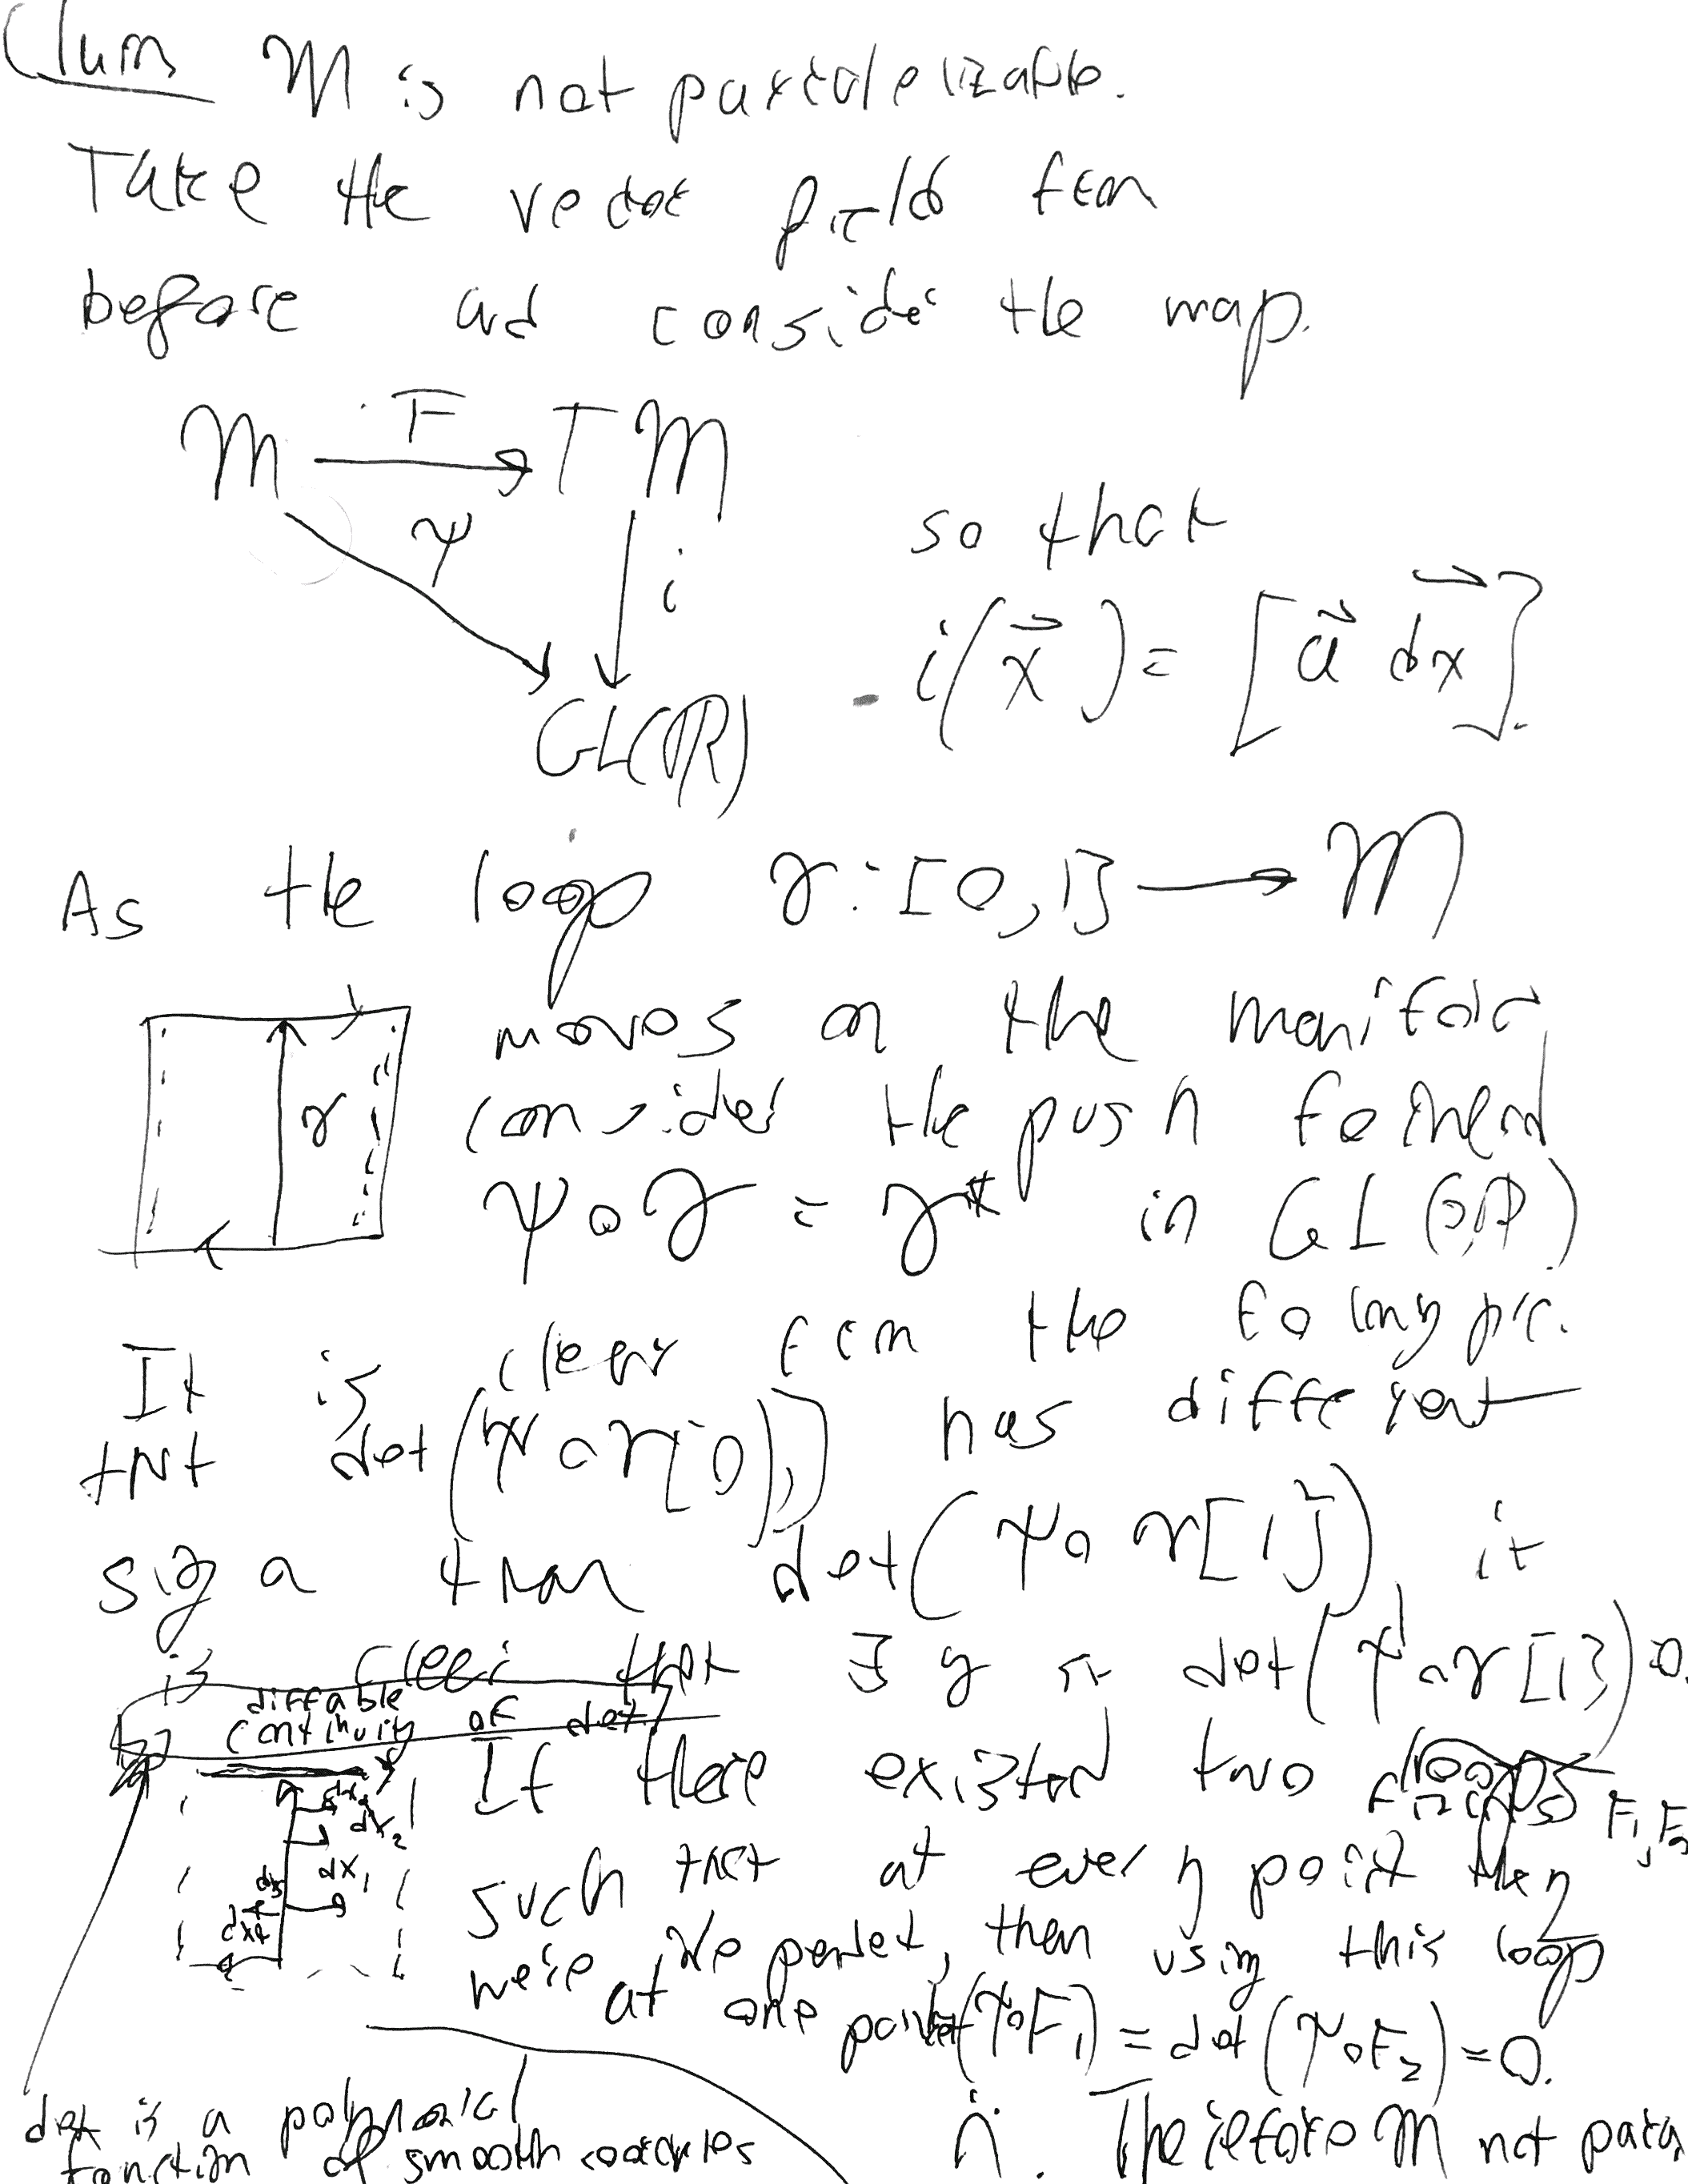
\includegraphics[width=\textwidth,height=\textheight]{image.png}

\end{document}\end
